\documentclass{standalone}
\usepackage{tikz}
\usepackage{ctex,siunitx}
\setCJKmainfont{Noto Serif CJK SC}
\usepackage{tkz-euclide}
\usepackage{amsmath}
\usepackage{wasysym}
\usetikzlibrary{patterns, calc}
\usetikzlibrary {decorations.pathmorphing, decorations.pathreplacing, decorations.shapes,}
\begin{document}
\small
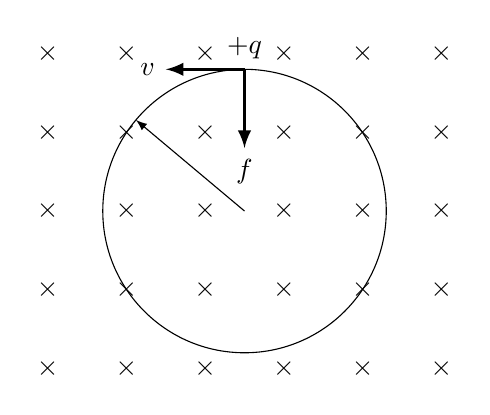
\begin{tikzpicture}[>=latex,scale=1]
	\foreach \x in {1,...,6}
	\foreach \y in {1,...,5}
	{
		\node at (\x,\y){$\times$};
	}
\draw (3.5,3) circle (1.8);

\draw [->, very thick](3.5,3+1.8)node[above]{$+q$}--(2.5,3+1.8)node [left]{$v$};
\draw [->, very thick](3.5,3+1.8) -- (3.5,3+.8)node[below]{$f$};
\draw [->](3.5,3)--+(140:1.8);
\end{tikzpicture}
\end{document}